\documentclass[border=4pt,12pt]{standalone}
% House style for redrawn exam diagrams (diagram-v4: 0.4pt lines, filled -latex arrows, fine dashes; stipple and hatching drawn as real dots/lines (no PDF/SVG patterns, so they render in every browser and at any scale); transparent background). Every figure \input's this.
\usepackage{amsmath,amssymb}
\usepackage{txfonts}
\usepackage{pdfrender,xcolor}
% \halo{text}: label on shading. The shading stops just around each letter's outline (a thin knock-out that follows the
% glyphs, like the papers' typesetting), never a box. Owner: "I don't want a box around the text".
\newcommand{\halo}[1]{\leavevmode\rlap{\pdfrender{TextRenderingMode=2,LineWidth=2.2pt,LineJoinStyle=1,StrokeColor=white,FillColor=white}#1}#1}
\usepackage{tikz,pgfplots}
\pgfplotsset{compat=1.18}
\usetikzlibrary{arrows.meta,calc,angles,quotes,patterns,patterns.meta,intersections,positioning,decorations.markings,shapes.geometric}
% Stipple and hatching are drawn as actual dots / lines clipped to the region (path picture), NOT as pattern fills:
% SVG <pattern> fills vanish or blur when browsers scale the image, so the owner could not see the shading.
% Each dot is a 0.72pt square (keeps SVGs small; reads as a dot at print size). Dots sit on one global staggered grid, so neighbouring regions line up.
\makeatletter
\newdimen\ex@x \newdimen\ex@y \newdimen\ex@xa \newdimen\ex@ya \newdimen\ex@xb \newdimen\ex@yb \newcount\ex@row
\def\exam@stipplecolor{black!75}\def\exam@dotr{0.42pt}\def\exam@dotgap{2.5}
\def\ex@rowdots{\ifdim\ex@x<\ex@xb \pgfpathrectangle{\pgfqpoint{\dimexpr\ex@x-0.36pt\relax}{\dimexpr\ex@y-0.36pt\relax}}{\pgfqpoint{0.72pt}{0.72pt}}\advance\ex@x by \exam@dotgap pt\relax\expandafter\ex@rowdots\fi}
\def\exam@stipple{%
  \pgftransformreset% dots are sized in real points even inside scaled pictures
  \pgfpointanchor{path picture bounding box}{south west}\ex@xa=\pgf@x \ex@ya=\pgf@y
  \pgfpointanchor{path picture bounding box}{north east}\ex@xb=\pgf@x \ex@yb=\pgf@y
  \pgfsetfillcolor{\exam@stipplecolor}\pgfmathsetmacro\ex@h{\exam@dotgap/2}%
  \pgfmathtruncatemacro\ex@r{floor(\ex@ya/\ex@h)-1}\ex@row=\ex@r\relax
  \ex@y=\ex@r\dimexpr\ex@h pt\relax
  \loop\ifdim\ex@y<\ex@yb
    \pgfmathtruncatemacro\ex@c{floor(\ex@xa/\exam@dotgap)-1}\ex@x=\ex@c\dimexpr\exam@dotgap pt\relax
    \ifodd\ex@row \advance\ex@x by \ex@h pt\fi
    \ex@rowdots
    \advance\ex@y by \ex@h pt \advance\ex@row by 1
    \ifnum\numexpr\ex@row-(\ex@row/4)*4\relax=0 \pgfusepath{fill}\fi% flush every 4 rows: bounded TeX memory, few clip copies in the SVG
  \repeat\pgfusepath{fill}}
\newdimen\ex@d
\def\exam@hatch#1{% #1 = 1 for /, -1 for \ ; lines 45 degrees, 3pt apart
  \pgftransformreset
  \pgfpointanchor{path picture bounding box}{south west}\ex@xa=\pgf@x \ex@ya=\pgf@y
  \pgfpointanchor{path picture bounding box}{north east}\ex@xb=\pgf@x \ex@yb=\pgf@y
  \ex@d=\dimexpr\ex@yb-\ex@ya\relax \ex@x=\dimexpr\ex@xa-\ex@d\relax
  \loop\ifdim\ex@x<\ex@xb
    \ifnum#1>0 \pgfpathmoveto{\pgfqpoint{\ex@x}{\ex@ya}}\pgfpathlineto{\pgfqpoint{\dimexpr\ex@x+\ex@d\relax}{\ex@yb}}%
    \else \pgfpathmoveto{\pgfqpoint{\ex@x}{\ex@yb}}\pgfpathlineto{\pgfqpoint{\dimexpr\ex@x+\ex@d\relax}{\ex@ya}}\fi
    \advance\ex@x by 4.24pt
  \repeat
  \pgfsetlinewidth{0.4pt}\pgfsetstrokecolor{black}\pgfusepath{stroke}}
\def\examstipple{\exam@stipple}\def\examhatch{\exam@hatch}\def\examsetstipplecolor#1{\def\exam@stipplecolor{#1}}\def\examsetdotgap#1{\def\exam@dotgap{#1}}
\makeatother
% (legacy pattern kept for old files)
% staggered stipple like the NESA papers' dotted shading
\pgfdeclarepatternformonly{exam stipple}{\pgfpointorigin}{\pgfqpoint{2.2pt}{2.2pt}}{\pgfqpoint{2.2pt}{2.2pt}}{%
  \pgfpathcircle{\pgfqpoint{0.55pt}{0.55pt}}{0.42pt}\pgfpathcircle{\pgfqpoint{1.65pt}{1.65pt}}{0.42pt}\pgfusepath{fill}}
\tikzset{
  every picture/.style={line width=0.6pt, >={Latex[length=2mm,width=1.3mm]}},
  curve/.style={line width=0.6pt},
  open arrow/.style={-{Latex[length=2mm,width=1.3mm]}},  % owner: filled -latex heads everywhere, no open chevrons
  aux/.style={dash pattern=on 2pt off 1.5pt, line width=0.6pt},
  shade/.code={\def\exA{#1}\def\exB{none}\ifx\exA\exB\else\pgfkeysalso{fill=black!18}\fi},
  shade/.default=on,
  shade dots/.style={fill=none, path picture={\examstipple}},
  stipple color/.code={\examsetstipplecolor{#1}},
  stipple gap/.code={\examsetdotgap{#1}},
  shade dense dots/.style={fill=none, stipple gap=1.6, path picture={\examstipple}},
  shade hatch/.style={fill=none, path picture={\examhatch{1}}},
  shade hatch reverse/.style={fill=none, path picture={\examhatch{-1}}},
  shade solid/.style={fill=black},
  pt/.style={circle, fill, inner sep=1.1pt},
  open pt/.style={circle, draw, fill=white, inner sep=1.1pt},
}
\pgfplotsset{
  exam axes/.style={axis lines=middle, axis line style={->}, xlabel={$x$}, ylabel={$y$},
    xlabel style={anchor=west}, ylabel style={anchor=south}, tick label style={font=\small},
    every axis plot/.append style={line width=0.6pt, black}, samples=200, clip=false,
    enlargelimits=false, axis on top},
}

\begin{document}
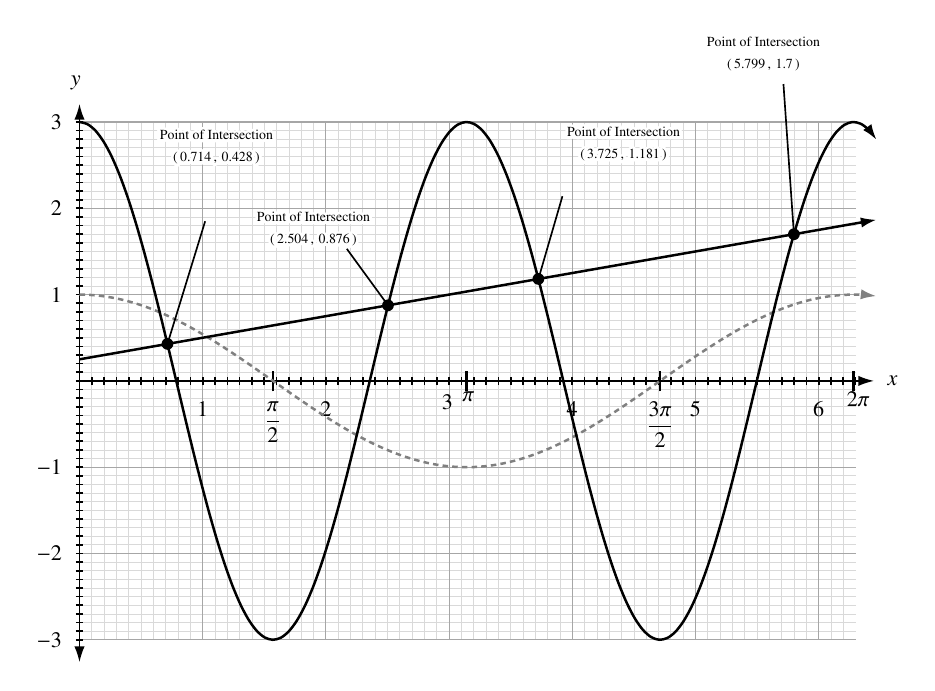
\begin{tikzpicture}[x=1.5646cm,y=1.096cm]
\draw[black!15,line width=0.3pt] (0,-3) grid[xstep=0.1,ystep=0.1] (6.3,3);
\draw[black!35,line width=0.4pt] (0,-3) grid[step=1] (6.3,3);
\draw[->] (0,0) -- (6.45,0);
\draw[<->] (0,-3.26) -- (0,3.21);
\foreach \i in {1,...,63} \draw (\i/10,-0.05) -- (\i/10,0.05);
\foreach \j in {-30,...,30} \draw (-0.03,\j/10) -- (0.03,\j/10);
\foreach \t in {pi/2,pi,3*pi/2,2*pi} \draw[line width=0.9pt] (\t,-0.12) -- (\t,0.12);
\node[font=\footnotesize,anchor=west] at (6.47,0) {$x$};
\node[font=\footnotesize] at (-0.03,3.45) {$y$};
\foreach \i in {1,2,4,5,6} \node[font=\footnotesize,anchor=north] at (\i,-0.12) {$\i$};
\node[font=\footnotesize,anchor=north east,inner sep=1pt] at (3.06,-0.12) {$3$};
\node[font=\footnotesize,anchor=north west,inner sep=1pt] at (3.08,-0.08) {$\pi$};
\node[font=\footnotesize,anchor=north west,inner sep=1pt] at (6.2,-0.08) {$2\pi$};
\node[font=\footnotesize,anchor=north] at (pi/2,-0.13) {$\dfrac{\pi}{2}$};
\node[font=\footnotesize,anchor=north] at (3*pi/2,-0.13) {$\dfrac{3\pi}{2}$};
\foreach \j in {-3,-2,-1,1,2,3} \node[font=\footnotesize,anchor=east] at (-0.06,\j) {$\j$};
\draw[aux,line width=0.9pt,black!50,->] plot[smooth,domain=0:6.47,samples=90] (\x,{cos(\x r)});
\draw[line width=0.9pt,->] (0,0.25) -- (6.47,{(6.47+1)/4});
\draw[line width=0.9pt,->] plot[smooth,domain=0:6.47,samples=100] (\x,{3*cos(2*\x r)});
% intersections
\foreach \p in {0.714,2.504,3.725,5.799} \node[pt,inner sep=1.5pt] at (\p,{(\p+1)/4}) {};
\draw (1.02,1.85) -- (0.714,0.428);
\draw (2.17,1.53) -- (2.504,0.876);
\draw (3.92,2.14) -- (3.725,1.181);
\draw (5.714,3.44) -- (5.799,1.7);
\node[font=\tiny,align=center] at (1.112,2.711) {\halo{Point of Intersection}\\[2pt]\halo{$(\,0.714\,,\,0.428\,)$}};
\node[font=\tiny,align=center] at (1.899,1.761) {\halo{Point of Intersection}\\[2pt]\halo{$(\,2.504\,,\,0.876\,)$}};
\node[font=\tiny,align=center] at (4.416,2.746) {\halo{Point of Intersection}\\[2pt]\halo{$(\,3.725\,,\,1.181\,)$}};
\node[font=\tiny,align=center] at (5.552,3.789) {Point of Intersection\\[2pt]$(\,5.799\,,\,1.7\,)$};
\end{tikzpicture}
\end{document}